\chapter{Kravspecifikation}\label{kapitel_KS}

\begin{longtabu} to \linewidth{@{}l l l X[j]@{}}
    Version &    Dato &    Ansvarlig &    Beskrivelse\\[-1ex]
    \midrule
    0.1 &    9/9-15 &    Alle &    Oprettelse af dokument\\
    1.0 &    21/9-15 &    LB, JL, HR, RR, SV &    Tilføjelse af use case "\textit{Log ind}", samt amå-rettelser efter møde med vejleder\\
    1.1 &    23/9-15 &    Alle &    Rettelser af "\textit{Log ind}"\ use case, samt rettelser af andet i KS\\
    2.0 &    28/9-15 &    Alle &    Tilføjer ny use case, "\textit{Kalibrer systemet}", og tilretter "\textit{Log ind}"\ use case\\
2.1	&	29/9-15	&	Alle	& 	\\
3.0	&	7/10-15	&	Alle	&	Tilrettelser efter review med gr. 4\\   
\label{version_KS}
\end{longtabu}

\textbf{Formål}\\
Formålet med en kravspecifikation er, at beskrive systemets funktionelle og ikke-funktionelle krav til kunden. Kravspecifikationen er kontrakten mellem virksomhed og kunde.\\

\section{Systembeskrivelse}
Dette program skal opfylde de obligatoriske krav, opstillet af IHA:
\begin{itemize}
\item Programmet skal programmeres i C$\#$
\item Programmet skal kunne kalibrere blodtrykssignalet og foretage en nulpunktsjustering
\item Blodtrykket skal vises kontinuert på en graf i GUI, hvor der ses systolisk og diastolisk tryk
\item Målingerne skal kunne gemmes som tekstfil eller i database
\item Systemet skal kunne filtrere blodtrykket i selve programmet via et digitalt filter, dette skal kunne slås til og fra.
\end{itemize}
Ud fra projektets vision, beskrevet i projektformuleringen, skal der udvikles et system til måling af blodtryk. Systemet skal kunne bruges på computere, der forudsættes at have adgang til måleudstyret, og samtidig overholder de opstillede krav.
\\
Systemet skal kunne tilsluttes et væskefyldt kateter og vise en blodtrykskurve på en computerskærm. 
\\
Systemet skal indeholde et elektronisk kredsløb, som forstærker signalet fra trykstransduceren og filtrerer det med et indbygget analogt filter. 
\\
Systemet skal indeholde et program, som kan vise blodtrykket som funktion af tiden. Dette foregår ved, at målingerne indlæses fra blodtryksmåleren, omdannes til et digitalt signal vha. DAQ, indlæses i et C$\#$-program og vises grafisk.

\section{Funktionelle krav}


\subsection{Aktør-kontekstdiagram}
Der er udarbejdet et aktør-kontekst diagram med tilhørende aktørbeskrivelser, hvor de forskellige aktører i systemet er angivet og beskrevet.

\begin{figure}[H]
\centering
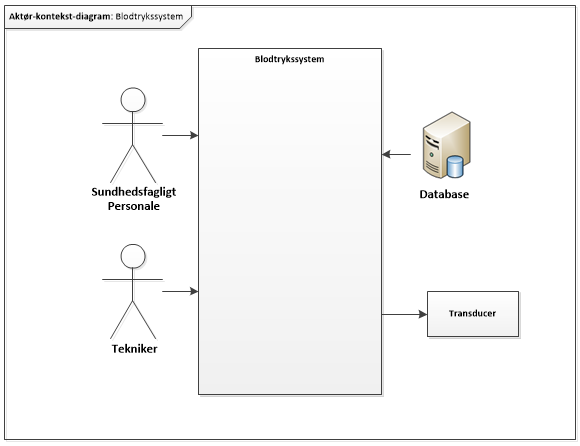
\includegraphics[scale=0.90]{ak.PNG}
\caption{Aktør-kontekstdiagram}
\end{figure}

\newpage

\subsection{Aktørbeskrivelse}

\begin{longtabu} to \linewidth{@{}l l X[j]@{}}
    \textbf{Aktørnavn} &        \textbf{Type} &    \textbf{Beskrivelse}\\[-1ex]
    \midrule
    Sundhedsfagligt personale &    Primær &    Aktøren starter, foretager og afslutter målingen. Aktøren skal have relevans i henhold til en operationsstue samt have kendskab til proceduerne herved\\
    Patient &        Sekundær &    Aktørens blodtryk undersøges ved at tilslutte blodtryksmålesystemet til patientens arterier.\\
    Database &        Sekundær &    Måledataene gemmes i databasen.\\
    Tekniker &       Sekundær &    Kalibrerer systemet\\
    
\caption{Aktørbeskrivelse.}\\
\label{actortable}
\end{longtabu}


\subsection{Use case-diagram}
Der er ud fra de overordnede, definerede krav til projektet, udviklet et use case-diagram. Diagrammet viser aktørerne i systemet, samt de fire scenarier der er valgt at fokusere på i dette system. 

\begin{figure}[H]
\centering
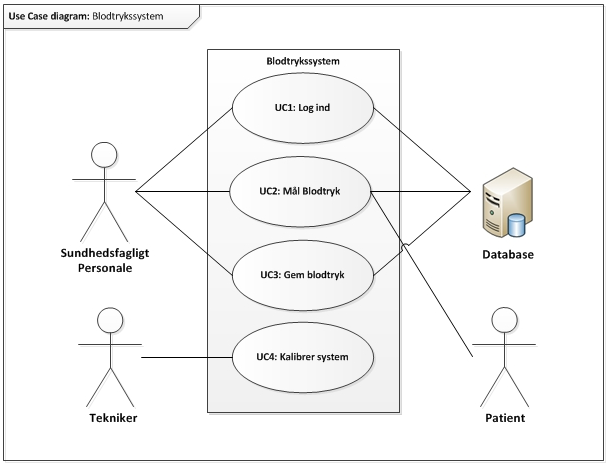
\includegraphics[scale=0.90]{uc.PNG}
\caption{Use case diagram}
\end{figure}



\subsection{Use cases}
Ud fra use case-diagrammet, er der udarbejdet en fully-dressed use case til hvert scenarie. Disse indgår herunder. 
\\

%% ----------------Use Case 1----------------------------

\begin{longtabu} to \linewidth{@{}l r X[j]@{}}
\toprule
    {\large \textbf{Use case 1 - Log ind}} && \\
    \toprule
    Navn &&    Log ind\\
    Scenarie &&    Hovedscenarie\\
    Use case ID &&    UC1\\
    Primær aktør &&    Sundhedsfagligt personale\\
    Sekundær aktør(er) &&    Database\\
    Initialisere &&    Sundhedsfagligt personale trykker på \textit{"Log ind"}-knap\\
    Mål &&    Sundhedsfagligt personale er logget ind og klar til at foretage måling.\\
    Forudsætninger &&    Systemet er operationelt\\
    Resultat &&    Sundhedsfagligt personale er succesfuldt logget ind i systemet.\\
    \toprule
    
    Hovedforløb &    1. &    Sundhedsfagligt personale indtaster ID\\[-1ex]
                &    2. &    Sundhedsfagligt personale indtaster tilhørende password\\[-1ex]
                &    3. &    Sundhedsfagligt personale trykker på \textit{"Log ind"}-knappen\newline
                			[3a. \textit{Fejl i indtastede ID eller password}]\\[-1ex]
                &	4.	&	Automatisk nulpunktsjustering foretages\\[-1ex]
                            
    \toprule
    Undtagelser &    3a. & [\textit{Fejl i indtastede ID eller password}] \\[-1ex]
    & 1. &  Systemet gør opmærksom på fejl, og lader bruger indtaste password og ID igen\\[-1ex]
                \toprule
   
\caption{Fully dressed Use case 1}
\label{UC1}
\end{longtabu}
\newpage

%% ----------------------Use Case 2----------------------------

\begin{longtabu} to \linewidth{@{}l r X[j]@{}}
\toprule
    {\large \textbf{Use case 2 - Mål blodtryk}} && \\
    \toprule
    Navn &&    Mål blodtryk\\
    Scenarie &&    Hovedscenarie\\
    Use case ID &&    UC2\\
    Primær aktør &&    Sundhedsfagligt personale\\
    Sekundær aktør(er) &&    Patient, database\\
    Initialisere &&    Efter UC1 er kørt succesfuldt\\
    Mål &&    At overvåge patientens blodtryk og vise dette kontinuert på en graf\\
    Forudsætninger &&    UC1 er kørt succesfuldt. Sundhedsfagligt personale har placeret intraarteriel nål i patienten\\
    Resultat &&    Sundhedsfagligt personale kan aflæse blodtryk i form af en kontinuerlig graf på GUI.\\
    \toprule
    Hovedforløb &    1. &    Sundhedsfagligt personale indtaster patientens CPR-nummer\\[-1ex]
    			&    2. &    Sundhedsfagligt personale trykker på knappen \textit{"Hent patientoplysninger"}\newline
    			[2a. \textit{Det indtastede CPR-nummer er ikke gyldigt}]\\[-1ex]
                &    3. &    Systemet viser målingen kontinuert i en graf på GUI\newline
                [3a. \textit{Blodtryk er for højt eller lavt}]\\
                &    4. &    Sundhedsfagligt personale har mulighed for, på GUI'en, at vælge mellem funktionerne:\\[-1ex]
                &	a. &	"\textit{Med digitalt filter}"\\[-1ex]
                &	b.	&	"\textit{Uden digitalt filter}"\\[-1ex]
                             %[3a. \textit{Blodtryk er for højt/lavt og SP alarmeres.}]\newline
                             %[3a. \textit{Blodtryk er for højt/lavt og SP alarmeres}]\\[-1ex]
                %&    4. &    ...\\[-1ex]
    \toprule
    Undtagelser &    2a. &    [\textit{Det indtastede CPR nummer er ikke gyldigt}]\\[-1ex]
    &	1. &	Systemet gør bruger opmærksom på fejl, og beder om ny indtastning af CPR nummer\\[-1ex]
    &	3a.	&	[\textit{Blodtryk er for højt eller lavt}]\\[-1ex]
    &	1.	&	Systemet alarmerer sundhedsfagligt personale\\[-1ex]
    &	2.	&	Sundhedsfagligt personale har nu mulighed for at slå systemets alarm på "\textit{Lydløs}"\- -tilstand i en periode på tre minutter\\[-1ex]
    &	3.	&	Alarmen stopper ved normalisering af blodtrykket\\
                \toprule
       
  
\caption{Fully dressed Use case 2}
\label{UC2}
\end{longtabu}
\newpage

%% --------------------------Use Case 3---------------------

\begin{longtabu} to \linewidth{@{}l r X[j]@{}}
\toprule
    {\large \textbf{Use Case 3 - Gem data}} && \\
    \toprule
    Navn &&    Gem data\\
    Scenarie &&    Hovedscenarie\\
    Use case ID &&    UC3\\
    Primær aktør &&    Sundhedsfagligt personale\\
    Sekundær aktør(er) &&    Database, tekniker\\
    Initialisere &&    Sundhedsfagligt personale\\
    Mål &&    At gemme måledataene i en database\\
    Forudsætninger &&    UC2 er gennemført\\
    Resultat &&    Måledata er gemt korrekt i databasen\\
    \toprule
    Hovedforløb &    1. &    Sundhedsfagligt personale trykker på "\textit{Gem data}"\- -knappen\\[-1ex]
                %&    2. &   ....\\[-1ex]
                &    2. &    Måledata gemmes i databasen\\[-1ex]
                             %[3a. \textit{...}]\newline
                             %[2a. \textit{Måledata kan ikke gemmes}]\\[-1ex]
                %&    4. &    ....\\[-1ex]
                &    3. &    Systemet giver beskeden: "\textit{Data gemt}"\\[-1ex]
                             %[3a. \textit{Data ikke gemt}]\\
 %   Undtagelser &    2a. &    [\textit{Måledata kan ikke gemmes}]\\[-1ex]
  %  &	1.	&	Der kommer en pop-up meddelelse "\textit{Data er ikke gemt}"\\[-1ex]
   % &	2.	&	Sundhedsfagligt personale trykker "\textit{OK}"\ og UC3 starter fra punkt 1\\
   % &	3.	&	Efter tre forsøg tilkaldes tekniker automatisk\\ 
                %&    3b. &    ....\\[-1ex]
                %&    5a. &    ....\\
                \toprule
\caption{Fully dressed Use case 3}
\label{UC3}
\end{longtabu}
\newpage

%-------------------Use case 4------------------------

\begin{longtabu} to \linewidth{@{}l r X[j]@{}}
\toprule
    {\large \textbf{Use Case 4 - Kalibrer system}} && \\
    \toprule
    Navn &&    Kalibrer system\\
    Scenarie &&    Hovedscenarie\\
    Use case ID &&    UC4\\
    Primær aktør &&    Tekniker\\
    Sekundær aktør(er) &&    \\
    Initialisere &&    Systemet\\
    Mål &&    At kalibrere systemet\\
    Forudsætninger &&    Tekniker er tilkaldt\\
    Resultat &&    Systemet er kalibreret\\
    \toprule
    Hovedforløb &    1. &    Tekniker påtrykker systemet tre kendte tryk\\[-1ex]
                &    2. &   Tekniker aflæser responserne på GUI\\[-1ex]
                &    3. &    Tekniker noterer afvigelserne fra de kendte tryk\newline
                             %[3a. \textit{...}]\newline
                             [3a. \textit{Der er ingen afvigelser}]\\[-1ex]
                %&    4. &    ....\\[-1ex]
                &    4. &   Tekniker kalibrerer afvigelsen i systemets software\\[-1ex]
                             %[5a. \textit{...}]\\
               &	5.	&	UC4 startes forfra\\[-1ex]
    \toprule
    Undtagelser &    3a. &    [\textit{Der er ingen afvigelse}]\\[-1ex]
    %&	1.	&	..\\[-1ex]
    &	1.	&	UC4 afsluttes\\
                %&    3b. &    ....\\[-1ex]
                %&    5a. &    ....\\
                \toprule
\caption{Fully dressed Use case 4}
\label{UC4}
\end{longtabu}
\newpage


\section{Ikke-funktionelle krav}

Ikke-funktionelle krav beskrevet ved FURPS+ med MoSCoW.

\subsection{FURPS+}
MoSCoW er angivet i en parantes med enten M, S, C eller W. 
\\

\textbf{Functionality}
\begin{enumerate}
\item (M) Programmet skal programmeres i C$\#$, Visual Studio
\item (S) Systemet bør kunne angive pulsen via en lyd ved hvert hjerteslag ved .... Hz
\item (M) Blodtrykket skal kunne gemmes i en database og skal indeholde 
\begin{enumerate} 
\item Patient-CPR, ansvarligt sundhedspersonale, ansvarlig organisation, dato
\item Rådata, samplerate (Hz), interval (s), data format, måleformat, starttid, antal målinger
\end{enumerate}
\item (M) Programmet skal kunne foretage en nulpunktsjustering 
\item (M) Blodtrykket skal måles indenfor 10 mmHg præcision
%\item (M) Systemet skal kunne filtrere blodtrykssignalet i selve programmet via et digitalt filter
%\begin{enumerate}
%\item (M) Dette skal kunne slås til og fra
%\end{enumerate} 

\noindent 
\textbf{Usability}
\item (M) Programmet skal indeholde en "\textit{Log ind}"\- -knap
\item (M) Programmet skal indeholde en "\textit{Hent patientoplysninger}"\- -knap
\item (M) Programmet skal indeholde en "\textit{Gem data}"\- -knap
\item (M) Programmet skal indeholde en "\textit{Lydløs}"\- -knap
%\item (S) Det bør være muligt at starte/stoppe uden at skulle genstarte programmet
%\item (M) Blodtrykket skal vises kontinuert i en graf på en GUI, hvor både diastolisk og systolisk tryk indgår

\textbf{Reliability}
\item (S) Systemet bør kunne køre fejlfrit i et år
\item (S) Systemet bør have en "mean time to restore" på højst 24 timer\\
Systemet får herved en tilgængelighed beregnet ved
$$Availability = \frac{MTBF}{MTBF+MTTR}=\frac{365}{365+1}= 0,997 = 99,7\%$$
MTBF = "mean time between failure" \\
MTTR = "mean time to restore"\\
\newpage

\textbf{Performance}
\item (M) Systemet skal kontinuert vise en grafisk afbildning af blodtrykket, hvor tryk er op af y-aksen og tiden er på x-aksen i intervallet af 6 sekunder 

\textbf{Supportability}
\item (S) Softwaren bør være opbygget af trelagsmodellen
%\item (M) Systemet skal kunne kalibreres af tekniker 

\textbf{+ Test conditions}
%\item (M) Der skal være adgang til en computer med Visual Studio og National Instrument
\end{enumerate}

\subsection{Skitse af system}

\begin{figure}[htb]
  \begin{minipage}{0.35\textwidth}
    \centering
      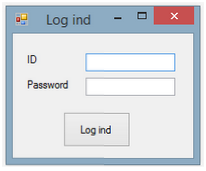
\includegraphics[width=\textwidth]{login.PNG}
      \caption{Log ind GUI}
    \label{fig:figur1}
  \end{minipage}
  \hspace{0.1\textwidth}
  \begin{minipage}{0.40\textwidth}
    \centering
      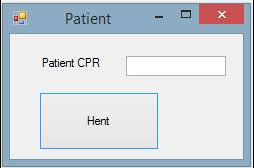
\includegraphics[width=\textwidth]{patient}
      \caption{Patient-id GUI}
    \label{fig:figur2}
  \end{minipage}
\end{figure}

\begin{figure}[H]
\centering
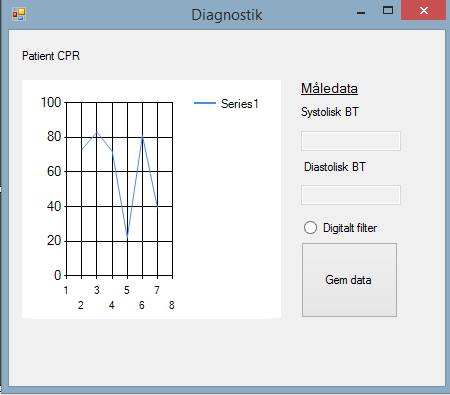
\includegraphics[scale=0.80]{dia.PNG}
\caption{Diagnose GUI}
\end{figure}

\begin{figure}[H]
\centering
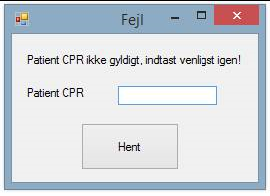
\includegraphics[scale=0.90]{fejl.PNG}
\caption{Fejl patient-CPR}
\end{figure}